\section{Scenario 1}
Alberto has to buy a new smartphone. He loves the services that his provider offers and he knows he can buy a new phone on its website.

\begin{enumerate}
	\item He goes on \url{www.tim.it}
	\item He clicks on "PRODOTTI" \url{www.tim.it/prodotti}
	\item In the smartphone section he can choose between smartphone or iPhone. He clicks on "iPhone" \url{www.tim.it/prodotti/smartphone-e-telefoni/iphone}
	\item Alberto sees that there are no promotions on iPhone so he goes back by clicking on "PRODOTTI"
	\item There is a promotion on Samsung Galaxy S8. He clicks on "SCOPRI" \url{www.tim.it/prodotti/smartphone-e-telefoni/samsung-galaxy-s8}
	\item He looks for the price and the specs. Alberto is interested and he wants to buy this phone. He clicks on "ACQUISTA". He is redirected on the ecommerce website of TIM and the purchase is continued through this site
\end{enumerate}

\newpage

\subsection{Results}
\begin{enumerate}
	
%------------------------------------------------------------------------------------------------------
	
\item Report on \url{www.tim.it}

\begin{center}
	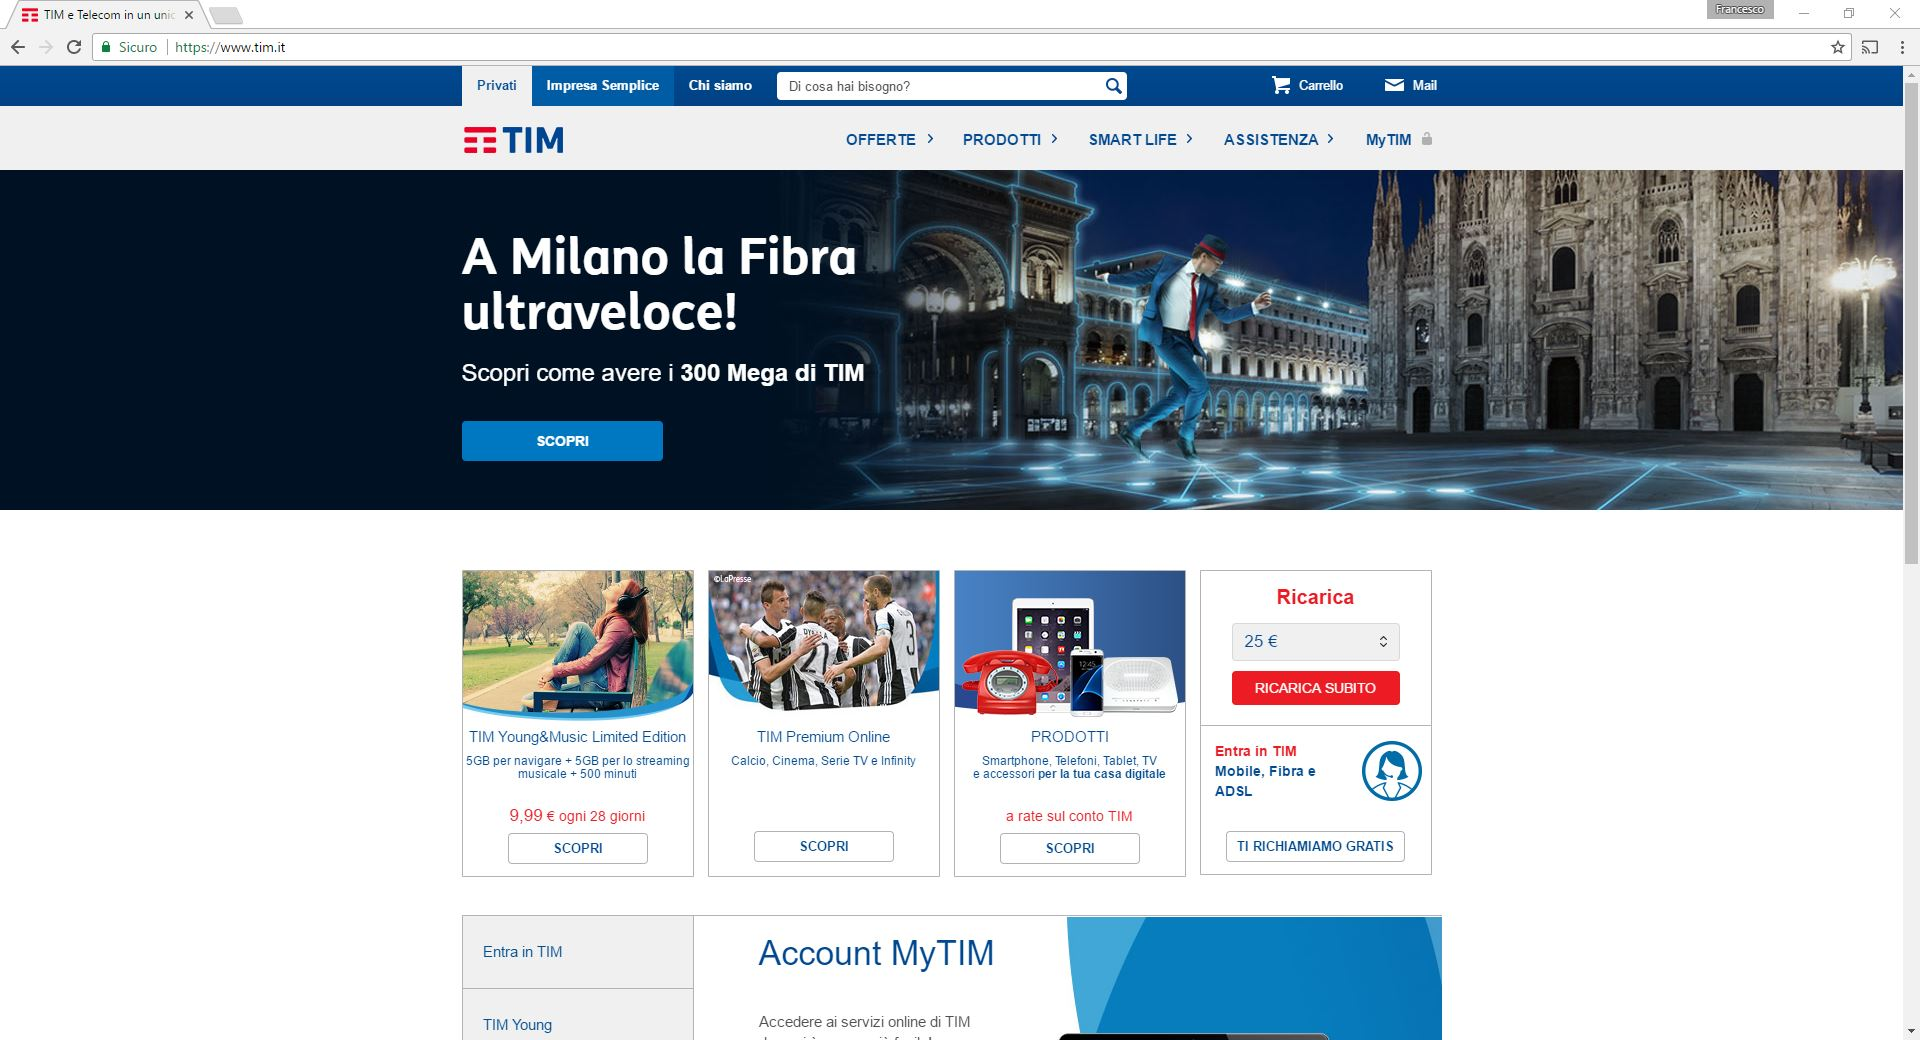
\includegraphics[width=\textwidth]{Screenshot/homepage.jpg}
\end{center}
\vspace{1cm}

	\paragraph*{Content heuristics \\ Text}
	\begin{itemize}
		\item accuracy: satisfied
		\item currency: \textcolor{red}{severely violated}\\the user cannot know if the page is updated
		\item coverage: satisfied
		\item content objectivity: satisfied
		\item authority: satisfied
		\item conciseness: satisfied		
	\end{itemize}
	
	\paragraph*{General communication quality}
	\begin{itemize}
		\item text errors: satisfied
		\item multimedia consistency: satisfied
	\end{itemize}

	\paragraph*{Navigation heuristics \\ Navigation within a topic}
	\begin{itemize}
		\item segmentation: n/a
	\end{itemize}	
	
	\paragraph*{Navigation within a transition}
	\begin{itemize}
		\item transition list: n/a
	\end{itemize}
	
	\paragraph*{Navigation within a group of topics}
	\begin{itemize}
		\item introduction list: n/a
		\item group navigation: n/a
	\end{itemize}
	
	\paragraph*{Backward navigation}
	\begin{itemize}
		\item go back: n/a
	\end{itemize}
	
	\paragraph*{Overall navigation}
	\begin{itemize}
		\item landmarks: satisfied\\
		they are well visible on the top-right corner of the website
		\item link consistency: satisfied
		\item orientation clues: satisfied
		\item orientation clues - topic: n/a
		\item group orientation clues: n/a
		\item transition orientation clues: n/a
	\end{itemize}	
	
	\paragraph*{Visual and semantic heuristics \\ Overall graphic design }
	\begin{itemize}
		\item visual identity: satisfied\\
		the palette represents the colors of the company logo
		\item chromatic code consistency: satisfied
		\item background contrast: satisfied
		\item font size: satisfied
		\item font color: satisfied
		\item font type: satisfied
		\item anchor identity: satisfied\\
		several links are wrapped in buttons 
		\item anchor states: satisfied\\
		anchors change states when the user hovers on them
		\item icon consistency: satisfied
	\end{itemize}
	
	\paragraph*{Page layout}
	\begin{itemize}
		\item visual proximity: satisfied
		\item layout conventions: satisfied
		\item semiotics: satisfied
	\end{itemize}	
	
	\paragraph*{Cognitive heuristics \\ Single page}
	\begin{itemize}
		\item information overload: \textcolor{orange}{partially violated}\\
		due to the number of services that the site offers, a novice could be overwhelmed by a lot of informations
	\end{itemize}	
	
	\paragraph*{Information architecture}
	\begin{itemize}
		\item classification adequacy within group of topics: n/a
		\item website mental map: satisfied
	\end{itemize}
\newpage
%------------------------------------------------------------------------------------------------------

\item Report on \url{www.tim.it/prodotti}

\begin{center}
	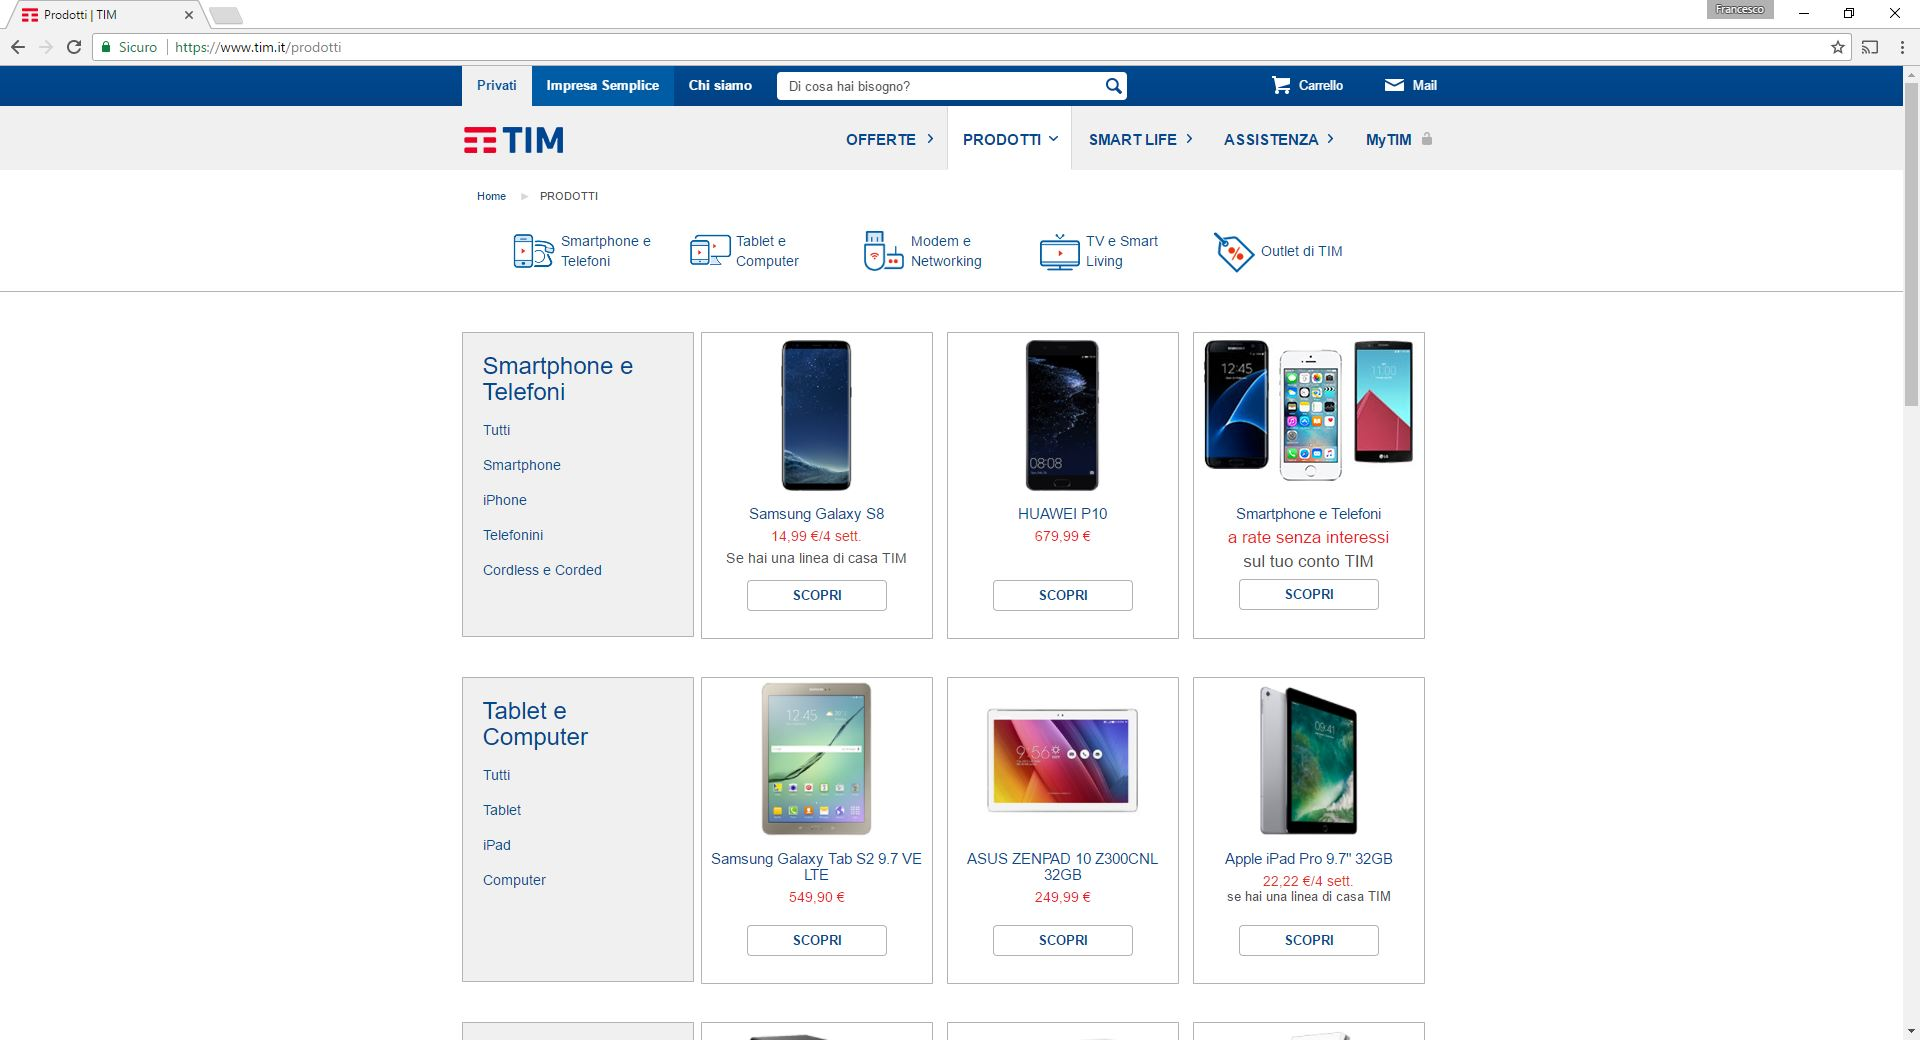
\includegraphics[width=\textwidth]{Screenshot/prodotti.jpg}
\end{center}
\vspace{1cm}

	\paragraph*{Content heuristics \\ Text}
	\begin{itemize}
		\item accuracy: satisfied
		\item currency: \textcolor{red}{severely violated}\\the user cannot know if the page is updated
		\item coverage: satisfied
		\item content objectivity: satisfied
		\item authority: satisfied
		\item conciseness: satisfied		
	\end{itemize}

	\paragraph*{General communication quality}
	\begin{itemize}
		\item text errors: satisfied
		\item multimedia consistency: satisfied
	\end{itemize}

	\paragraph*{Navigation heuristics \\ Navigation within a topic}
	\begin{itemize}
		\item segmentation: n/a
	\end{itemize}	
	
	\paragraph*{Navigation within a transition}
	\begin{itemize}
		\item transition list: n/a
	\end{itemize}
	
	\paragraph*{Navigation within a group of topics}
	\begin{itemize}
		\item introduction list: satisfied\\
		this site identifies several groups of topics ("Smartphone e Telefoni", "Tablet e Computer"...)
		\item group navigation: n/a
	\end{itemize}

	\paragraph*{Backward navigation}
	\begin{itemize}
		\item go back: \textcolor {orange}{partially violated}\\
		there isn't a "go back" functionality but the user can exploit the TIM logo to return to the homepage or select a position in the website structure path (Home $\triangleright$ PRODOTTI)
	\end{itemize}
	
	\paragraph*{Overall navigation}
	\begin{itemize}
		\item landmarks: satisfied\\
		they are well visible on the top-right corner of the website
		\item link consistency: satisfied
		\item orientation clues: satisfied\\
		under the logo there is a site structure path
		\item orientation clues - topic: n/a
		\item group orientation clues: n/a
		\item transition orientation clues: n/a
	\end{itemize}	
	
	\paragraph*{Visual and semantic heuristics \\ Overall graphic design }
	\begin{itemize}
		\item visual identity: satisfied
		\item chromatic code consistency: satisfied
		\item background contrast: satisfied
		\item font size: satisfied
		\item font color: satisfied
		\item font type: satisfied
		\item anchor identity: satisfied
		\item anchor states: satisfied
		\item icon consistency: satisfied
	\end{itemize}
	
	\paragraph*{Page layout}
	\begin{itemize}
		\item visual proximity: satisfied
		\item layout conventions: satisfied
		\item semiotics: satisfied
	\end{itemize}	
	
	\paragraph*{Cognitive heuristics \\ Single page}
	\begin{itemize}
		\item information overload: satisfied
	\end{itemize}	
	
	\paragraph*{Information architecture}
	\begin{itemize}
		\item classification adequacy within group of topics: n/a
		\item website mental map: satisfied
	\end{itemize}

\newpage

%------------------------------------------------------------------------------------------------------

\item Report on \url{www.tim.it/prodotti/smartphone-e-telefoni/iphone}

\begin{center}
	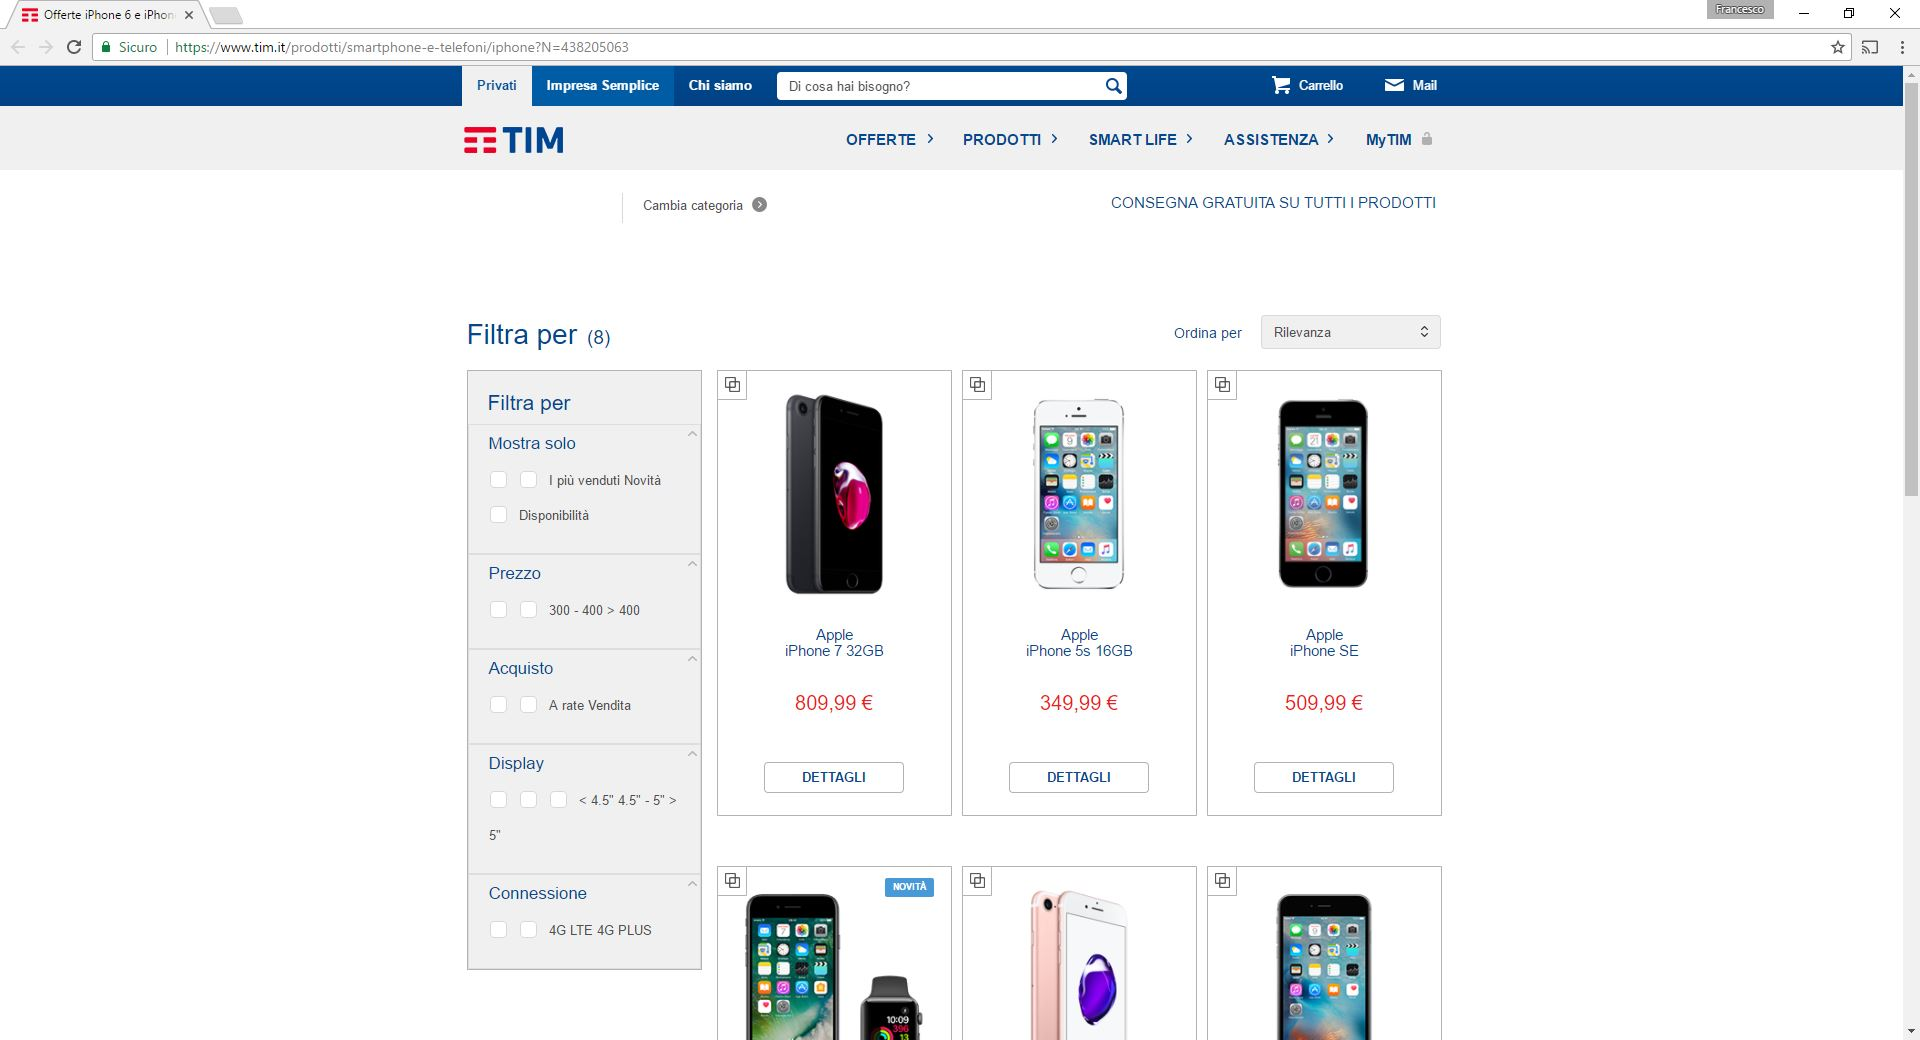
\includegraphics[width=\textwidth]{Screenshot/iphone.jpg}
\end{center}
\vspace{1cm}

	\paragraph*{Content heuristics \\ Text}
	\begin{itemize}
		\item accuracy: satisfied
		\item currency: \textcolor{red}{severely violated}\\the user cannot know if the page is updated
		\item coverage: satisfied
		\item content objectivity: satisfied
		\item authority: satisfied
		\item conciseness: satisfied		
	\end{itemize}
	
	\paragraph*{General communication quality}
	\begin{itemize}
		\item text errors: satisfied
		\item multimedia consistency: satisfied
	\end{itemize}
	
	\paragraph*{Navigation heuristics \\ Navigation within a topic}
	\begin{itemize}
		\item segmentation: n/a
	\end{itemize}	
	
	\paragraph*{Navigation within a transition}
	\begin{itemize}
		\item transition list: n/a
	\end{itemize}
	
	\paragraph*{Navigation within a group of topics}
	\begin{itemize}
		\item introduction list: n/a
		\item group navigation: satisfied\\
		from this page it is possible to reach every item of this group of topics
	\end{itemize}
	
	\paragraph*{Backward navigation}
	\begin{itemize}
		\item go back: \textcolor{red}{severely violated}\\
		there is no "go back" functionality, the user can go to the homepage through the TIM logo or repeat the steps by clicking "PRODOTTI"
	\end{itemize}
	
	\paragraph*{Overall navigation}
	\begin{itemize}
		\item landmarks: satisfied\\
		they are well visible on the top-right corner of the website 
		\item link consistency: satisfied
		\item orientation clues: \textcolor{red}{severely violated}\\
		the user cannot know where he/she is, there are no title nor path
		\item orientation clues - topic: n/a
		\item group orientation clues: \textcolor{red}{severely violated}\\
		the user cannot know which group of topics he/she is visiting ("Smartphone e Telefoni/iPhone")
		\item transition orientation clues: n/a
	\end{itemize}	
	
	\paragraph*{Visual and semantic heuristics \\ Overall graphic design }
	\begin{itemize}
		\item visual identity: satisfied
		\item chromatic code consistency: satisfied
		\item background contrast: satisfied
		\item font size: satisfied
		\item font color: satisfied
		\item font type: satisfied
		\item anchor identity: satisfied
		\item anchor states: satisfied
		\item icon consistency: satisfied
	\end{itemize}
	
	\paragraph*{Page layout}
	\begin{itemize}
		\item visual proximity: satisfied
		\item layout conventions: satisfied
		\item semiotics: satisfied
	\end{itemize}	
	
	\paragraph*{Cognitive heuristics \\ Single page}
	\begin{itemize}
		\item information overload: satisfied
	\end{itemize}	

	\paragraph*{Information architecture}
	\begin{itemize}
		\item classification adequacy within group of topics: satisfied
		\item website mental map: satisfied
	\end{itemize}

\newpage

%------------------------------------------------------------------------------------------------------

\item Report on \url{www.tim.it/prodotti/smartphone-e-telefoni/samsung-galaxy-s8}

\begin{center}
	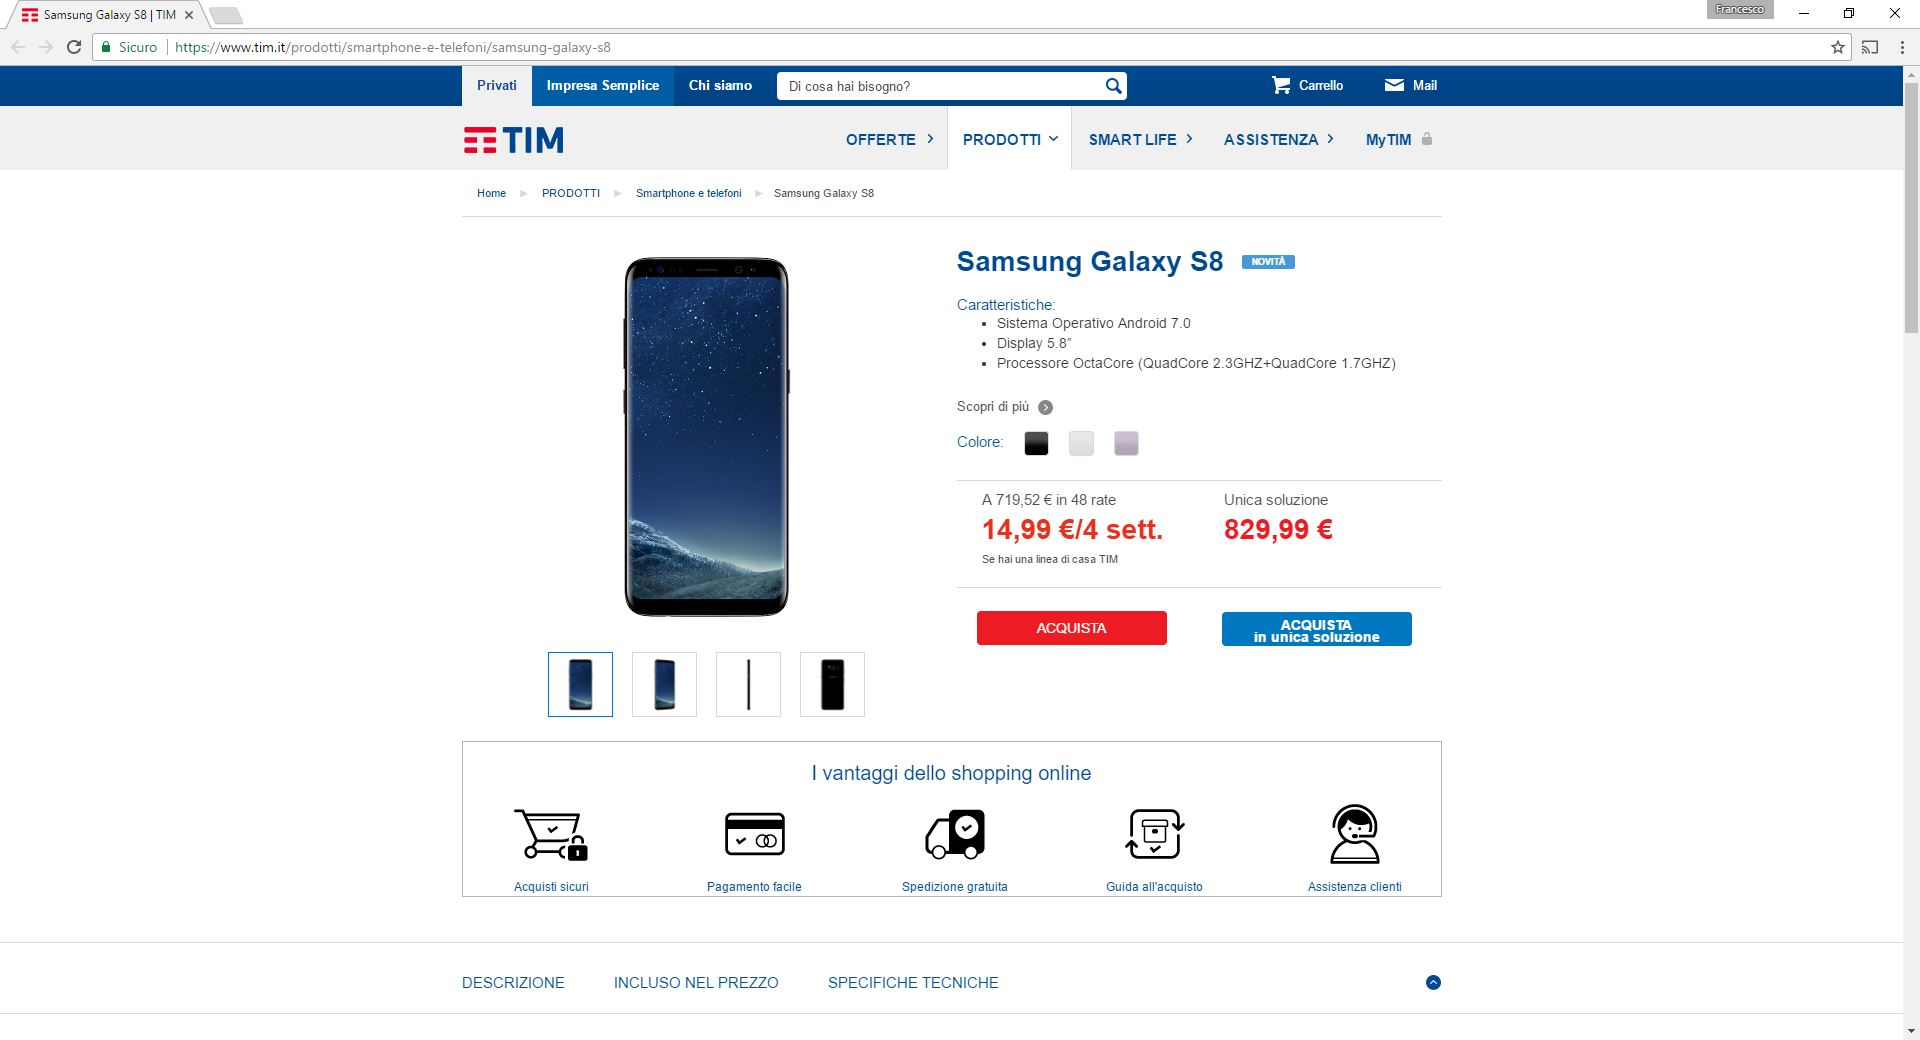
\includegraphics[width=\textwidth]{Screenshot/galaxys8.jpg}
\end{center}
\vspace{1cm}

	\paragraph*{Content heuristics \\ Text}
	\begin{itemize}
		\item accuracy: satisfied
		\item currency: \textcolor{red}{severely violated}\\the user cannot know if the page is updated
		\item coverage: satisfied
		\item content objectivity: satisfied
		\item authority: satisfied
		\item conciseness: satisfied		
	\end{itemize}

	\paragraph*{General communication quality}
	\begin{itemize}
		\item text errors: satisfied
		\item multimedia consistency: satisfied
	\end{itemize}

	\paragraph*{Navigation heuristics \\ Navigation within a topic}
	\begin{itemize}
		\item segmentation: satisfied\\
		the information of the topic are organized in sub-sections on the same page
	\end{itemize}	

	\paragraph*{Navigation within a transition}
	\begin{itemize}
		\item transition list: satisfied\\
		there are links related to other topics ("I vantaggi dello shopping online")
	\end{itemize}

	\paragraph*{Navigation within a group of topics}
	\begin{itemize}
		\item introduction list: n/a
		\item group navigation: \textcolor{orange}{partially violated}\\
		the user can reach the group by the site structure path but he/she can't reach items related to the group
	\end{itemize}

	\paragraph*{Backward navigation}
	\begin{itemize}
		\item go back: \textcolor{orange}{partially violated}\\
		there isn't a "go back" functionality but the user can exploit the TIM logo to return to the homepage or select a position in the website structure path (Home $\triangleright$ PRODOTTI $\triangleright$ Smartphone e Telefoni $\triangleright$ Samsung Galaxy S8)
	\end{itemize}

	\paragraph*{Overall navigation}
	\begin{itemize}
		\item landmarks: satisfied\\
		they are well visible on the top-right corner of the website
		\item link consistency: satisfied
		\item orientation clues: satisfied\\
		under the logo there is a site structure path
		\item orientation clues - topic: satisfied\\
		the user knows the subsection he/she is visiting. When the user navigate through the site, the section's labels are well visible on top of the page
		\item group orientation clues: satisfied
		\item transition orientation clues: satisfied
	\end{itemize}	

	\paragraph*{Visual and semantic heuristics \\ Overall graphic design }
	\begin{itemize}
		\item visual identity: satisfied
		\item chromatic code consistency: satisfied
		\item background contrast: satisfied
		\item font size: satisfied
		\item font color: satisfied
		\item font type: satisfied
		\item anchor identity: satisfied
		\item anchor states: satisfied
		\item icon consistency: satisfied
	\end{itemize}

	\paragraph*{Page layout}
	\begin{itemize}
		\item visual proximity: satisfied
		\item layout conventions: satisfied
		\item semiotics: satisfied
	\end{itemize}

	\paragraph*{Cognitive heuristics \\ Single page}
	\begin{itemize}
		\item information overload: satisfied
	\end{itemize}	

	\paragraph*{Information architecture}
	\begin{itemize}
		\item classification adequacy within group of topics: n/a
		\item website mental map: satisfied
	\end{itemize}
	\end{enumerate}
\newpage